\section{Method}
\label{sec:method}
In this section, we present our perception-guided neural scene synthesis for virtual reality. Based on a concentric spherical representation (\Cref{sec:method:representation}), our system predominantly comprises of two main steps: visual- and stereo- acuity adaptive view synthesis (\Cref{sec:synthesis}), and image-based real-time rendering to composite stereo display frames (\Cref{sec:method:blending}).
We then craft an analytical spatial-temporal model to guide the optimization of our intra-system variables for desired precision-performance balance (\Cref{sec:method:optimization}).
\begin{figure}
    \centering
    \includegraphics[width=0.96\linewidth]{TOG/figs/parameters.pdf}
    % \subfloat[Notations]{\includegraphics[width=0.96\linewidth]{TOG/figs/parameters.pdf}\label{fig:variables}}
    
    % \subfloat[Correlation between loss and parameters]{\includegraphics[width = 0.96\linewidth]{example-image-a}}
    \caption{Coordinate system and variable annotations.}
    \label{fig:notations}
\end{figure}
\subsection{Egocentric Neural Representation}
\label{sec:method:representation}
The recent single-object-oriented ``outside-in'' view synthesis methods \cite{sitzmann2019deepvoxels,mildenhall2020nerf} typically represent the training targets using uniform voxelization. However, immersive VR environments introduce open challenges for such parameterization due to the rapid variation of the egocentric (first-person) viewing (e.g., \Cref{fig:teaser:scene}).
As a consequence, the neural representation on large virtual environments typically suffer from ghosting artifacts, low resolution, or slow speed (e.g., the right triangle in \Cref{fig:teaser:quality}).
%We tailor our method specifically for egocentric (first-person) views in immersive VR environments.
%rendering of immersive viewer-centered ``inside-out'' scenes is challenging owing to the rapid variation of scene content. 
\paragraph{Egocentric coordinates}
To tackle this problem we are inspired by the recent panorama dis-occlusion methods \cite{Lin:DeepPanorama,Benjamin:2020:RTV,Broxton:immersiveLF} to depict the rapidly varying first-person views with concentric spheres. This representation enables robust rendering at real-time rates and allows for 6DoF interaction to navigate complex immersive environments. 
As visualized in \Cref{fig:notations}, our representation is parameterized with the number of concentric spheres ($\sphereNum$) and their respective radii ($\mathbf{\sphereRadius}=\{\sphereRadius_i\},i\in [1,\sphereNum]$). Our network aims at predicting the function $\mlpFunc(\hat{\SpatialPt})\triangleq(r,g,b,d)$ of any position $\mathbf{\hat{\SpatialPt}}({\sphereRadius_{i,i\in[1,\sphereNum]},\theta,\phi})$ on these $\sphereNum$ spherical surfaces. %\dnc{$\mathbf{q}$ may be more proper}\qisun{Just to avoid confusion with \Cref{fig:notations}. What do you think?}\dnc{Then perhaps we can use $\hat{q}$ as shown in \Cref{fig:notations} I think the alphabet 'q' means it's in spherical system, 'p' never exists anywhere else}
Here, $(r,g,b)$ and $d$ are the predicted color and density, respectively. 
We then employ a ray marching through this intermediate function to produce images of specified views.

\paragraph{Training and synthesis}
%\dnc{Perhaps we can merge this paragraph with above section? And move the last paragraph of above section to here as a intro. Then this section is more focusing on GAZE-AWARE}
For each scene, we approximate the function $\mlpFunc$ by training a multilayer perceptron (MLP) network, similar to \cite{mildenhall2020nerf}.
The network is composed of $\mlpLayerNum$ fully-connected layers of $\mlpChannelNum$ channels, each using ReLu as the activation function. We will further determine $\mlpLayerNum$, $\mlpChannelNum$ and $\sphereNum$ via a spatial-temporal optimization in \Cref{sec:method:optimization}.
Once trained, the network achieves 4D prediction on the spherical voxels, on which a ray marching rendering is performed to synthesize the final frames for display.% based on users' frame-wise views. 
Similar to \cite{mildenhall2020nerf}, we apply a trigonometric input encoding and compute the L2-distance between the volume-rendered and mesh-rendered images as the training loss function. We discuss the specifics of training data creation and implementations in \Cref{sec:impl}.

\subsection{Gaze-Aware Acceleration}
\label{sec:synthesis}
\qisun{@nianchen: does this section title sounds reasonable to you?}
%The scene representation above is created to parameterize a given 3D space for neural synthesis. 
%the foveated rendering manner of VR display through training two orthogonal neural networks that are tailored for the perceptual acuity variances.
Our concentric spherical coordinate system, as described in \Cref{sec:method:representation}, addresses the view variance problem in VR. However, it sill suffers from significant rendering latency (seconds per frame). This is one of the core challenges causing neural representation to be unsuitable yet for VR. To combat the common performance problem of view synthesis, we predict multiple elemental images based on the viewer's real-time head and gaze motions\nothing{ instead of synthesizing a globally uniform image}. The elemental images are tailored for the visual acuity variances. We detail our network design and elemental image synthesis in the following section. We enable real-time responsiveness via introducing gaze-adaptive synthesis mechanisms.
\begin{figure}[bht]
    \centering
    \subfloat[fovea]{\includegraphics[width=0.3\linewidth]{TOG/figs/layer_blend/lobby_view0000_fovea.png}\label{fig:system:fovea}}\vspace{1em}
    \subfloat[mid-periphery]{\includegraphics[width=0.3\linewidth]{TOG/figs/layer_blend/lobby_view0000_mid.png}\label{fig:system:mid}}\vspace{1em}
    \subfloat[far-periphery]{\includegraphics[width=0.3\linewidth]{TOG/figs/layer_blend/lobby_view0000_periph.png}\label{fig:system:far}}
    
    \subfloat[rendering]{\includegraphics[width=0.9\linewidth]{TOG/figs/layer_blend/lobby_view0000_blendmask.png}\label{fig:system:blending}}
    \Caption{Synthesis output and rendering.}
    {%
    \subref{fig:system:fovea}/\subref{fig:system:mid}/\subref{fig:system:far} shows our individual gaze-contingent synthesis for fovea (within $20$deg)/mid-periphery (within $45$deg)/far-periphery(within $110$deg, the capability of our VR display), respectively. 
    \subref{fig:system:blending} illustrates our real-time rendering system by dynamically blending the individual images to the final displayed frame.
    }
    \label{fig:system}
\end{figure}
\paragraph{Adaptive visual acuity} 
%the user's current view $[\rayo,\camDir]$ and gaze position $\gazeDir$ that are tracked in real-time by a VR headset.
Existing neural scene representation networks predict uniform resolution images for offline third-person viewing.
Due to the trade-off between quality and latency during inference, they are typically executed with low quality and/or high latency when it comes large field-of-view and high resolution imagery. \praneeth{this line is confusing} 
Our method, without compromising performance, generates {\it perceptually} high quality frames matching the retinal acuity, i.e. how the retina perceives dynamic and stereo frames.
% Note that foveal/peripheral retinal images requires high/low pixel-wise precision but low/high FoV (number of pixels). Thus, we train two orthogonal neural networks that are tailored for the perceptual acuity variances. 
Because of foveation of imagery by the human visual system \cite{Guenter:2012:F3G}, we train two orthogonal networks (i.e., $\mlpFunc$s) to synthesize foveal ($\imageFoveal(\rayo,\camDir,\gazeDir)$, $0-20$deg), and peripheral elemental images (i.e., two $\mlpFunc$s to deploy for ray marching) for each eye.
The periphery includes mid- ($\imageMid(\rayo,\camDir,\gazeDir)$, $0-45$deg) and high- eccentricity visual fields ($\imageFar(\rayo,\camDir$), $0-110$deg), see \Cref{fig:system}.
Note that $\imageFar$ is independent from the gaze direction $\gazeDir$. 
%The images are defined as functions that maps individual camera rays ($\rayo,\rayd$) to an RGB color.
\dnc{Could move to section 4? I think it's implementation related}\qisun{I think the PDD numbers give readers a rough impression of the varied quality across each of the image, right?} Specifically, to incorporate the display hardware properties and perceptual effects, we define $\imageFoveal$/$\imageMid$/$\imageFar$ as of $128^2$/$256^2$/$230\times256$ resolutions respectively.
That is, the $\imageFoveal$ has the highest spatial resolution of $6.4$ pixels per degree (PDD), higher than those of $\imageMid$ ($5.7$ PDD) and $\imageFar$ ($2.33$ PDD).
%In each frame, the two networks independently return three elemental images, as seen from the separation range in deg, gradually larger areas along eccentricity. An example is shown in \Cref{fig:system}.

\paragraph{Adaptive stereo-acuity}
{
To be rendered on head-mounted displays, stereo elemental images $\imageFoveal^{\{l,r\}}$, $\imageMid^{\{l,r\}}$, and $\imageFar^{\{l,r\}}$ ($l$ and $r$ represent left and right eyes respectively) are required. This doubles the computational cost that is critical for latency- and frame-rate- sensitive VR experience  
\nothing{The separation of the three elemental images considers the varied visual acuity. However, in a head-mounted stereo VR displays, the rendered image are for two eyes, resulting in double computation for $\imageFoveal^{\{l,r\}}$, $\imageMid^{\{l,r\}}$, and $\imageFar^{\{l,r\}}$. Here $l$ and $r$ represent the projection images for left ($\rayo^l$) and right ($\rayo^r$) eyes respectively. 
Whereas, because $\imageMid^{\{l,r\}}$ and $\imageFar^{\{l,r\}}$ demand high spatial resolution due to their large eccentricity coverage, }
}
(please refer to \Cref{sec:study:intra} for detailed comparisons).

To tackle this problem towards real-time experience, we accommodate the inference process with the adaptive stereo-acuity in the periphery.
Specifically, besides the visual acuity, psychophysical studies have revealed human's significantly declined stereopsis while receding from the gaze point \cite{mochizuki2012magnitude}. Inspired this characteristic, instead of inferring $6$ elemental images, we perform the computation with $\imageFoveal^{\{l,r\}}$, $\imageMid^m$, and $\imageFar^m$, where $m$ indicates the view at the midpoint of the left and right eyes. The individual images are further blended for display, as detailed in \Cref{sec:method:blending}. 
\Cref{fig:mono} visualizes the stereo changes from the adaptation.
\begin{figure}[hb]
    \centering
    %\subfloat[w/o gaze-adaptive stereo]{\includegraphics[width=0.248\linewidth]{TOG/figs/stereo_periphery/bedroom_view0000_blended_stereo.png}\label{fig:mono:wo}}
    %\subfloat[w/ gaze-adaptive stereo]{\includegraphics[width=0.248\linewidth]{TOG/figs/mono_periphery/bedroom_view0000_blended_stereo.png}%\label{fig:mono:w}}
    %\subfloat[w/o gaze-adaptive stereo]{\includegraphics[width=0.248\linewidth]{TOG/figs/stereo_periphery/gallery_view0000_blended_stereo.png}\label{fig:mono:wo}}
    %\subfloat[w/ gaze-adaptive stereo]{\includegraphics[width=0.248\linewidth]{TOG/figs/mono_periphery/gallery_view0000_blended_stereo.png}%\label{fig:mono:w}}
    
    \subfloat[w/o gaze-adaptive stereo]{\includegraphics[width=0.48\linewidth]{TOG/figs/stereo_periphery/stereo_periphery.pdf}\label{fig:mono:wo}}%\hspace{0.5em}
    \subfloat[w/ gaze-adaptive stereo]{\includegraphics[width=0.48\linewidth]{TOG/figs/stereo_periphery/mono_periphery.pdf}\label{fig:mono:w}}
    %\subfloat[w/o gaze-adaptive stereo]{\includegraphics[width=0.248\linewidth]{TOG/figs/stereo_periphery/gas_view0000_blended_stereo.png}\label{fig:mono:wo}}
    %\subfloat[w/ gaze-adaptive stereo]{\includegraphics[width=0.248\linewidth]{TOG/figs/mono_periphery/gas_view0000_blended_stereo.png}\label{fig:mono:w}}
    
    %\subfloat[w/o gaze-adaptive stereo]{\includegraphics[width=0.248\linewidth]{TOG/figs/stereo_periphery/gas_view0001_blended_stereo.png}\label{fig:mono:wo}}
    %\subfloat[w/ gaze-adaptive stereo]{\includegraphics[width=0.248\linewidth]{TOG/figs/mono_periphery/gas_view0001_blended_stereo.png}\label{fig:mono:w}}
    \Caption{Visualization of the adaptive stereo-acuity with anaglyph.}
    {%
    \subref{fig:mono:wo} shows the rendered image with 6 retinal sub-images ($\imageFoveal^{\{l,r\}}$, $\imageMid^{\{l,r\}}$, and $\imageFar^{\{l,r\}}$).
    \subref{fig:mono:w} shows the rendered image with our adaptive and accelerated inference considering foveated stereoacuity ($\imageFoveal^{\{l,r\}}$, $\imageMid^{\{m\}}$, and $\imageFar^{\{m\}}$). Our method preserves full stereopsis in the fovea while reducing the angular resolution in the periphery for accelerated inference.
    }
    \label{fig:mono}
\end{figure}

\subsection{Real-Time Frame Composition}\dnc{May be moved to section 4 (merge with the paragraph 'Integration'). I think it's not closely related to our methodology and we have no key contributions about that. It's more like an engineering issue}\qisun{This whole section? I was concerned that would break the method completeness. Intentionally kept it short according to contribution level here.}
\label{sec:method:blending}
In real-time, we perform a image-based rendering that blends the elemental images. The output frames are rendered on the stereo VR displays.
To accommodate the uniformized $\imageMid^m$, we shift it with $-/+ \frac{\rayo^r-\rayo^l}{2}$ for left/right eye respectively. 
\dnc{Not accurate. shifting is related to mean of fovea depthmap inferred in actual implementation to minimize the misalignment between fovea and mid}
{
With the obtained elemental images as input, a fragment shader is executed to generate final images for each eye. Two adjunct layers are blended using a smoothstep function across $40\%$ of inner layer.
\nothing{After obtaining the individual images, our fragment shader retrieves the three frames and applied a pixel wise bilinear interpolation at each $10\%$ connecting areas between two adjunct layers.}
}
This enhances visual consistency on the edges between layers \cite{Guenter:2012:F3G}.
Moreover, to further preserve peripheral elemental images' visual fidelity due to its low PDD, we enhance the contrast following the mechanism of \cite{Patney:2016:TFR}, the details are visualized in \Cref{fig:method:blending}. %\dnc{Note: the contrast enhancement is performed on elemental images, before blending. Different enhancement parameters are applied for fovea, mid and periph layers}

\begin{figure*}[htb]
    \centering
    \subfloat[network overlay]{\includegraphics[width = 0.3\linewidth]{TOG/figs/system/overlap2.pdf}\label{fig:method:blending:overlay}}\hspace{1em}
    \subfloat[blending]{\includegraphics[width = 0.3\linewidth]{TOG/figs/system/blended2.pdf}\label{fig:method:blending:blending}}\hspace{1em}
    \subfloat[contrast enhance]{\includegraphics[width = 0.3\linewidth]{TOG/figs/system/blended_enhanced2.pdf}\label{fig:method:blending:contrast}}
    \Caption{Our multi-layer real-time rendering system.}
    {%
    \subref{fig:method:blending:overlay} shows the original 3-layer image output overlaid.
    \subref{fig:method:blending:blending} shows the result with cross-layer blending that enables smooth appearance on the edges.
    \subref{fig:method:blending:contrast} shows the contrast-enhanced rendering pass in the periphery.
    }
    \label{fig:method:blending}
\end{figure*}

\subsection{Latency-Quality Joint Optimization}
\label{sec:method:optimization}
As a view synthesis system based on sparse egocentric representation (the density of $\sphereNum$ spheres) and neural networks (the $\mlpLayerNum\times\mlpChannelNum$), the method inevitably introduces approximation errors. On the other hand, these variables also determine the online computational time that involves inferring function $\mlpFunc$ and ray marching the $\sphereNum$ spheres. 
However, VR strictly demands both quality and performance. We present a spatial-temporal model that analytically depicts the correlations and optimizes the variables for ideal user experience.

\paragraph{Precision loss of a 3D scene}
As shown in \Cref{fig:notations}, under the egocentric representation, a 3D point $\pt$ is re-projected as the nearest point on a sphere that connects it to the origin point:
\begin{equation}\label{eq:closestPoint3D}
{\pt^\prime}(\sphereNum,\mathbf{\sphereRadius},\SpatialPt) \triangleq \sphereRadius_k \frac{\pt}{\norm{\pt}}, \ k=\argmin_{j\in[1,\sphereNum]}\left(\norm{\norm{\SpatialPt}-\sphereRadius_j}\right).
\end{equation}

Similar to volume-based representation, the multi-spherical system is also defined in discrete domain. The sparsity thus naturally introduces approximation error that compromises the synthesis quality. To analytically model the precision loss, we investigate the geometric relationship among the camera, the scene, and the representation.
As illustrated in \Cref{fig:teaser:scene,fig:notations},  for a sphere (located at origin point) with radius $\sphereRadius$, its intersection (if exists) with a directional ray $\{\rayo,\rayd\}$ is
\begin{equation}
\intersectionFunc(\sphereRadius,\rayo,\rayd) = \rayo + \left({\left((\rayo\cdot\rayd)^2-\norm{\rayo}^2+\sphereRadius^2\right)}^{\frac{1}{2}}-\rayo\cdot\rayd\right)\rayd,
\label{eq:raySphereIntersection}
\end{equation}
where $\rayo$ and $\rayd$ are the ray's origin point and normalized direction respectively.
% \begin{equation}
% \left\{\intersectionFunc(\sphereRadius_i,\rayo,\rayd) \right\}\ |\ i\in[1,2,\dots,\sphereNum].
% \end{equation}
Inversely, given a view point $\rayo$ observing a spatial location $\SpatialPt$ represented in spherical coordinates, the ray connect them is with the direction $\rayd(\SpatialPt,\rayo)=\frac{\SpatialPt-\rayo}{\norm{\SpatialPt-\rayo}}$. This ray may intersect with more than one spheres. Among them, the closest one to $\SpatialPt$ is:
\begin{equation}\label{eq:closestPointImg}
\begin{aligned}
    \hat{\pt}&(\rayo,\sphereNum, \mathbf{\sphereRadius},\SpatialPt) \triangleq \\
    &\intersectionFunc(\sphereRadius_k,\rayo,\rayd(\SpatialPt,\rayo))\ |\ k=\argmin_{j\in[1,\sphereNum]}\left(\norm{\norm{\SpatialPt}-\sphereRadius_j}\right).
\end{aligned}
\end{equation}
In the 3D space, the offset distance $\norm{\pt^\prime-\hat{\pt}}$ indicates the precision loss at $\pt$ from the representation. By integrating over all view and scene points, we obtain:
\begin{equation}
\begin{aligned}
\sparseError(\sphereNum, \mathbf{\sphereRadius})  &= \iint \norm{\pt^\prime(\sphereNum,\mathbf{\sphereRadius},\SpatialPt)-\hat{\pt}(\rayo,\sphereNum, \mathbf{\sphereRadius},\SpatialPt)} \mathbf{d}\SpatialPt \mathbf{d}\rayo,\\
&\forall \{\rayo, \SpatialPt\} \text{ pair without occlusion in between}.
\label{eq:sparseError}
\end{aligned}
\end{equation}
$\sparseError$ depicts how the generic representation precision of a scene, given a coordinate system defined by $\sphereNum$ and $\mathbf{\sphereRadius}$.

In comparison, a neural representation aims at predicting projected image given a camera position $\rayo$ and orientation $\camDir$. Thus, we further extend \Cref{eq:sparseError} to image space to analyze the error given a set of camera's projection matrix  $\projectionMatrix(\rayo,\camDir)$ as
%However, typical 3D representations are not uniformly distributed points. Moreover, the network only predicts pixel colors/intensities but not depth. By extending \Cref{eq:sparseError} to the captured image space data, we obtain
\begin{align}
\imgSpaceError(\sphereNum, \mathbf{\sphereRadius}, \rayo, \camDir)  = \int \norm{\projectionMatrix(\rayo,\camDir)\cdot\left(\SpatialPt-
\hat{\pt}(\rayo,\sphereNum, \mathbf{\sphereRadius},\SpatialPt)\right)}\mathbf{d}\SpatialPt.
\label{eq:imageError}
\end{align}
From \Cref{fig:notations,eq:imageError}, we observe:
given a fixed min/max range of $\mathbf{\sphereRadius}$, $\sphereNum$ is negatively correlated to $\imgSpaceError$;
with a fixed $\sphereNum$, the correlation between distribution of $\sphereRadius_j$ and scene content (i.e., distribution of $\SpatialPt$s) also determines $\imgSpaceError$.

However, for neural scene representation, infinitely enlarging $\sphereNum$ would significantly raise the challenges in training precision and inference performance.
Likewise, increasing prediction and rendering densities (i.e., higher $\sphereNum$ or $\mlpLayerNum$/$\mlpChannelNum$) naturally improves the image output quality for lower \Cref{eq:imageError} while significantly increases the computation during ray marching, causing quality drop stretched along time. In the performance-sensitive VR scenario, the latency breaks the continuous viewing experiment and may cause simulator sickness. Thus, we determine the coordinate variables with a content-aware optimization towards optimal quality-speed performance.

\paragraph{Spatial-temporal modeling}
Inspired by \cite{Li:2020:TSP,albert2017latency}, we perform a spatial-temporal joint modeling to determine the optimal coordinate system ($\sphereNum$ and $\mathbf{\sphereRadius}$) for positional precision and MLP settings ($\mlpLayerNum$/$\mlpChannelNum$) for color precision that adapt to individual computational resources and scene content. This is achieved via a latency-precision modeling in the spatial-temporal domain.
%Specifically, we model the prediction image $P$ with gaze position ($G$) at time $t$ as $P_G(t)$ and the ground truth retinal image (from a simulated local rendering) as $\hat{P}_G(t)$.
%In practice, increasing the number of spheres $\sphereNum$ or number of MLP layers may affect the computational and transmissional latency but will improve the quality of individual frames (as in \Cref{eq:imageError}). Thus, we define the perceptual error as:
\begin{equation}
\begin{aligned}
\finalError(\sphereNum, &\mlpLayerNum, \mlpChannelNum) = 
\sum_t\int \mlpFunc_{\mlpLayerNum, \mlpChannelNum}(\SpatialPt)\times\\ &\norm{\projectionMatrix(\rayo_t,\camDir_t)\cdot\SpatialPt-\projectionMatrix(\rayo_{t-\latency},\camDir_{t-\latency})\cdot\pt(\sphereRadius_k,\rayo_{t-\latency},\rayd_{t-\latency})}\mathbf{d}\SpatialPt,
%&\int  \norm{ \imgSpaceError(\sphereNum, \mathbf{\sphereRadius}, \rayo_t, \rayd_t) - \imgSpaceError(\sphereNum, \mathbf{\sphereRadius}, \rayo_{t-l(\sphereNum, \mathbf{\sphereRadius})}, \rayd_{t-l(\sphereNum, \mathbf{\sphereRadius})})) } \mathbf{d} t
\label{eq:error:image}
\end{aligned}
\end{equation}
where $\latency\triangleq\latency(\sphereNum, \mlpLayerNum, \mlpChannelNum)$ is the system latency with a given coordinate and network setting.
$\mlpFunc_{\mlpLayerNum, \mlpChannelNum}(\SpatialPt)$ is the L1-distance between the four channels ($r$,$g$,$b$,$a$) and0 the highest values of network layer settings. For simplicity, we assumed uniformly distributed $\mathbf{\sphereRadius}$ with a fixed range of the spherical coverage.

Suggested by Albert et al. \shortcite{albert2017latency}, the latency for a foveated system shall reach below \textasciitilde$50$ms for undetectable artifacts. Given our test device's eye-tracking latency \textasciitilde$12ms$ and the photon submission latency \textasciitilde$14ms$ (\cite{albert2017latency}), the synthesis and rendering latency shall be less than $L_0 = 24$ms.
Thus, we determine the optimal $\{\sphereNum, \mathbf{\sphereRadius}\}$ to balance latency and precision as
\begin{equation}
\begin{aligned}
    &\argmin_{\sphereNum, \mlpLayerNum, \mlpChannelNum} \finalError(\sphereNum, \mlpLayerNum, \mlpChannelNum), \\
    & s.t.\ {l(\sphereNum, \mathbf{\sphereRadius})} < L_0
\end{aligned}
\end{equation}
\Cref{fig:optimization} visualizes an example of the optimization mechanism for in fovea. The optimized results ($\sphereNum, \mlpLayerNum, \mlpChannelNum$) for individual networks are detailed in the next section. The visual quality is validated by psychophysical study (\Cref{sec:study:user}) and objective analysis (\Cref{sec:study:quality}). The latency breakdown of our system is reported in \Cref{sec:study:intra}.
\begin{figure}[htb]
    \centering
    \subfloat[quality]{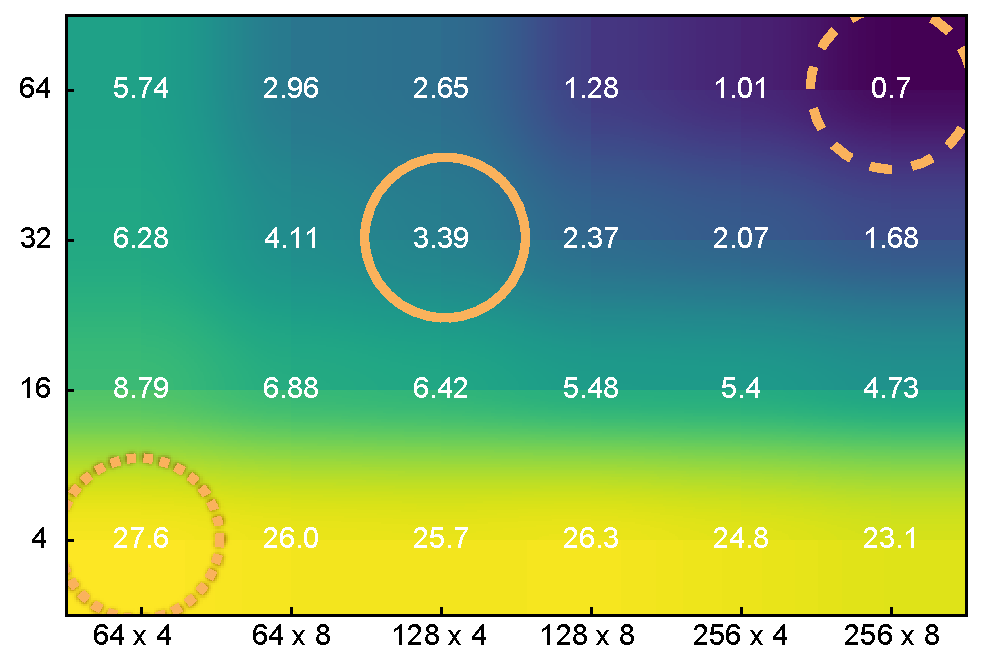
\includegraphics[width=0.48\linewidth]{TOG/figs/latency_vs_quality/heat_quality2.pdf}\label{fig:optimization:heat:quality}}
    \subfloat[latency]{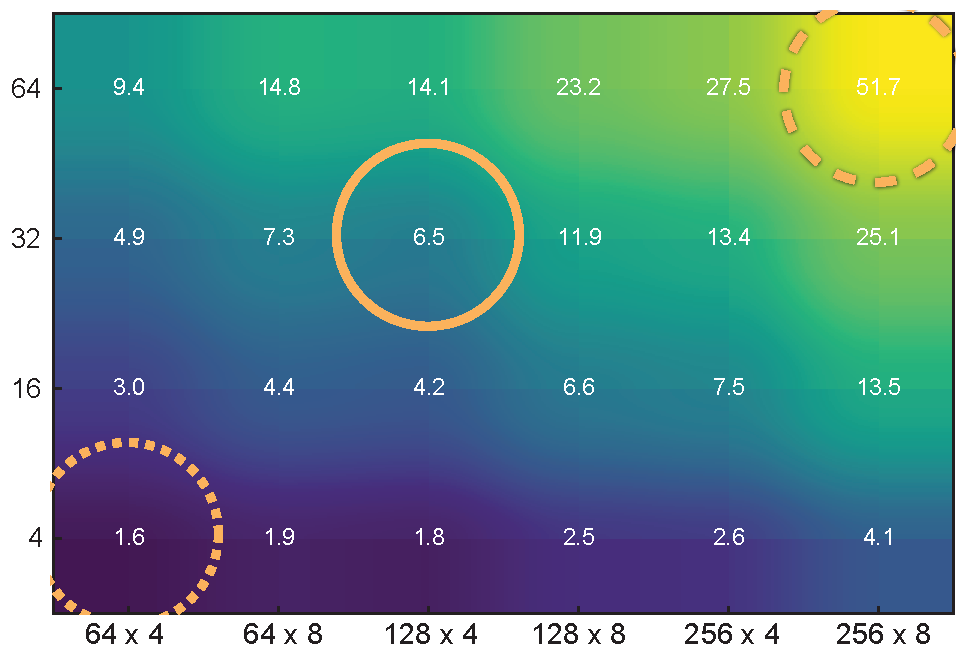
\includegraphics[width=0.48\linewidth]{TOG/figs/latency_vs_quality/heat_time2.pdf}\label{fig:optimization:heat:time}}
    
    \subfloat[quality-only]{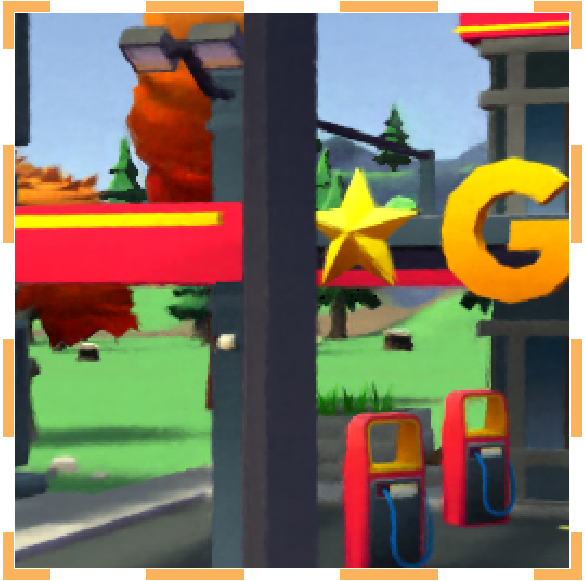
\includegraphics[width=0.3\linewidth]{TOG/figs/latency_vs_quality/quality_only.pdf}\label{fig:optimization:quality}}\hspace{0.5em}
    \subfloat[latency-only]{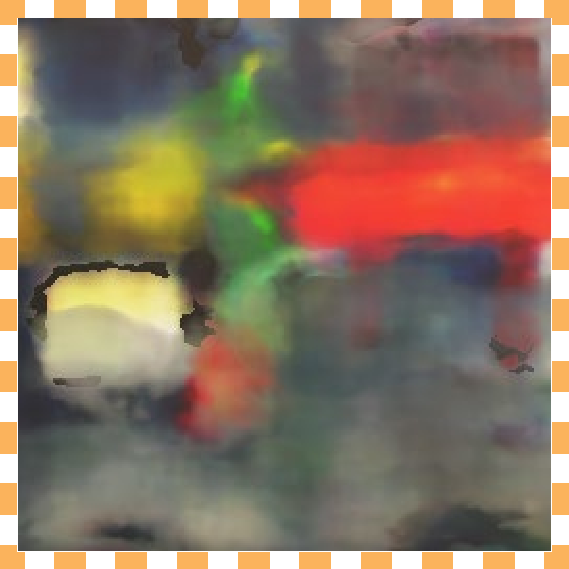
\includegraphics[width=0.3\linewidth]{TOG/figs/latency_vs_quality/latency_only.pdf}\label{fig:optimization:time}}\hspace{0.5em}
    \subfloat[ours]{\includegraphics[width=0.3\linewidth]{TOG/figs/latency_vs_quality/our.pdf}\label{fig:optimization:our}}
    \Caption{Latency-quality joint-optimization.}
    {%
    \protect\subref{fig:optimization:heat:quality}/\protect\subref{fig:optimization:heat:time} shows \protect\Cref{eq:imageError}/latency(in millisecond under pytorch implementation) of an example foveal network.
    The values are computed with various settings of $\mlpLayerNum\times\mlpChannelNum$ (x-axis) and $\sphereNum$ (y-axis). The second row indicates a corresponding foveal image under different settings. Our method balances both perceptual quality and latency.\nothing{\qisun{(Jan 24) What is the unit of \subref{fig:optimization:heat:time}? It shouldn't be second, right?}\dnc{It's millisecond.}}%nothing
    }
    \label{fig:optimization}
\end{figure}
\section{Implementation}\label{sec:impl}
In this section, we elaborate on how we collect data for training, the specific parameters that we choose for two orthogonal neural networks, and system integration.

\paragraph{Data generation}
For each scene, we trained two independent neural networks: foveal and periphery. We sampled the rendered view for two networks accordingly. To train the foveal neural network, we rendered an image of resolution $256^2$ per 20 deg. For periphery neural network, we rendered an image of resolution $256^2$ per $60$ deg. We repeated the above every $5$ cm on each axis.
% \nothing{
%\paragraph{Input encoding}
Similar to \cite{mildenhall2020nerf}, we also extend the input dimensions ($d=3$) to a higher dimensional ($d=60$) for training. 
\nothing{This is achieved via coding the input as:
\begin{align}
\iota (p) = (\sin(2^0 p), \cos(2^0 p), ..., \sin(2^{L-1}p, \cos(2^{L-1}p))
\label{eqn:inputencode}
\end{align}
The function $\iota (\cdot)$ is applied to dimension of $\SpatialPt=(r_\SpatialPt,\theta_\SpatialPt, \phi_\SpatialPt)$.
In our experiment we choose $L=10$.\qisun{What is $L$?}\dnc{It's an encoding parameter for input. maps 3D input to $R^{6L}$ space, as \autoref{eqn:inputencode} shows}
}
\paragraph{Optimized network variables}
Following the optimization results from \Cref{sec:method:optimization}, we implemented both foveal and periphery neural network with $\mlpLayerNum=128$ and $\mlpChannelNum=4$ , and $\sphereNum = 32$ for foveal network and $\sphereNum = 16$ for periphery network. We will discuss the visual quality and performance difference in ~\Cref{sec:study:intra}. \nothing{We sampled the near foveal network and far foveal with $N_{sample}=16$ and $N_{sample}=16$, while we sampled the near ($1/distance < 0.5$) peripheral with $N_{sample}=8$,  $N_{channel}=64$,  $N_{layer}=4$ and far ($1/distance >= 0.5$) peripheral with $N_{sample}=8$,  $N_{channel}=128$,  $N_{layer}=4$.}
\nothing{
\dnc{Move to section 3.4 or just drop it (cause we have no detail analysis about the bound)? This small paragraph seems strange at here.}
\paragraph{Ray marching bounding}
For accelerating the performance and quality (as compared in \Cref{fig:method:bounding}), we bound the min/max of $\mathbf{\sphereRadius}$. The bounding range, together with $\sphereNum$, $\mlpLayerNum$ and $\mlpChannelNum$, are determined from a spatial-temporal optimization, as detailed in \Cref{sec:method:optimization}. %The bounding, however, may introduce subtle quality drop, as shown in \Cref{fig:method:bounding}.
\begin{figure}
    \centering
    \subfloat[w/o bounding]{\includegraphics[width = 0.47\linewidth]{TOG/figs/depth_without_bound.png}}\hspace{1em}
    \subfloat[w bounding]{\includegraphics[width = 0.47\linewidth]{TOG/figs/depth_with_bound.png}}
    \Caption{Comparison of ray marching bounding.}
    {%
    }
    \label{fig:method:bounding}
\end{figure}
}%nothing
\paragraph{Integration} \dnc{this paragraph seems similar to 3.3.}
The stereoacuity significantly drops beyond fovea \cite{mochizuki2012magnitude}.
Our system reaches interactive performance (around 30FPS) for the first design -- the same procedure is applied to each eye (the details are addressed in \Cref{sec:study:intra}). To archive real-time performance (around 50FPS), we implemented mono-periphery for better performance. For each frame, we infer the same mid- and far- peripheral images for left and right eyes from the camera pose of central eye. In \Cref{sec:study:user}, we evaluated mono-periphery for subjective and objective measurements as well as discuss the visual quality and performance difference in ~\Cref{sec:study:intra}.
% \warning{We conducted a preliminary study to investigate how users perceive mono-periphery.}

\paragraph{Environment}
The system was implemented through OpenGL framework using CUDA and accelerated by TensorRT with Intel(R) Xeon(R) Gold 6230R CPU @ 2.10GHz (256GB RAM) and one NVIDIA GTX 3090 graphics card.
For each scene, we trained around 200 epochs for experiment use (about a day).